\begin{figure}
    \centering
    \captionsetup[subfigure]{labelformat=empty}
\begin{subfigure}{.5\textwidth}
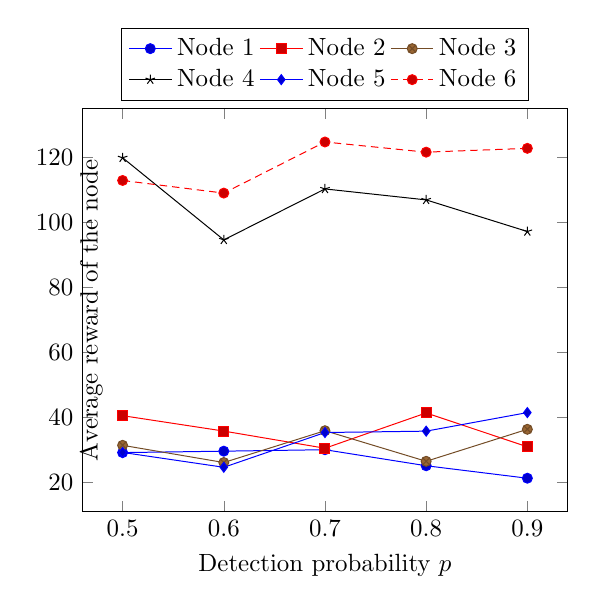
\begin{tikzpicture}[scale=0.9]
\begin{axis}[
  xlabel={Detection probability $p$},
  ylabel={Average reward of the node },
  y label style={at={(0.06,0.5)}},
  xtick={0.5,0.6,0.7,0.8,0.9,1.0},
  legend style={at={(0.5,1.2)},cells={align=right}, anchor=north,legend columns=3},
  grid style=dashed,
]

\addplot+[]
    coordinates {
(0.5,29.2207587022)(0.6,29.6591500811)(0.7,30.107769581)(0.8,25.1808225374)(0.9,21.3501334315)
};

\addplot+[]
    coordinates {
(0.5,40.5649596864)(0.6,35.8317201966)(0.7,30.5615817425)(0.8,41.4017616625)(0.9,31.0018428294)
};

\addplot+[]
    coordinates {
(0.5,31.4601711216)(0.6,26.1715912622)(0.7,35.9427616495)(0.8,26.5488358659)(0.9,36.3780765072)
};

\addplot+[]
    coordinates {
(0.5,119.788927983)(0.6,94.566243579)(0.7,110.212449824)(0.8,106.844518821)(0.9,97.138069126)
};

\addplot+[]
    coordinates {
(0.5,29.2697135288)(0.6,24.7098561839)(0.7,35.3909999115)(0.8,35.8083893589)(0.9,41.5087141375)
};

\addplot+[]
    coordinates {
(0.5,112.808511307)(0.6,108.932780706)(0.7,124.631408718)(0.8,121.507931814)(0.9,122.678991306)
};

\legend{Node 1, Node 2, Node 3, Node 4, Node 5, Node 6}
\end{axis}
\end{tikzpicture}

\caption{Scenario a)}
\label{fig:nodeimp_single}
\end{subfigure}
\begin{subfigure}{.33\textwidth}
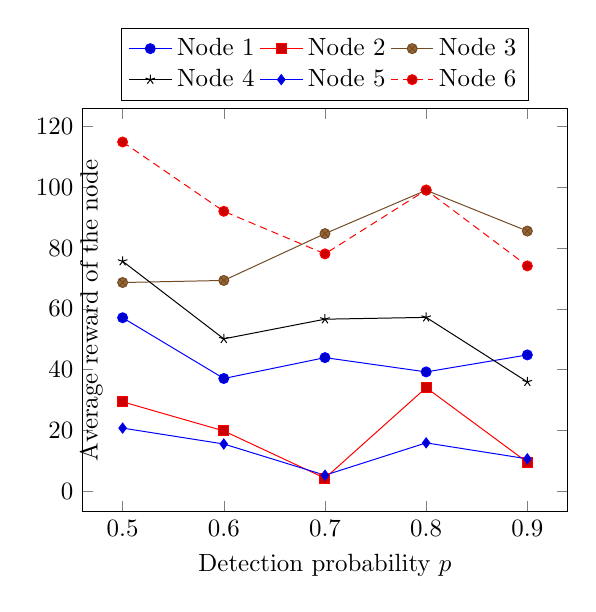
\begin{tikzpicture}[scale=0.9]
\begin{axis}[
  xlabel={Detection probability $p$},
  ylabel={Average reward of the node },
  y label style={at={(0.06,0.5)}},
  xtick={0.5,0.6,0.7,0.8,0.9,1.0},
  legend style={at={(0.5,1.2)},cells={align=right}, anchor=north,legend columns=3},
  grid style=dashed,
]

\addplot+[]
    coordinates {
(0.5,57.0711574474)(0.6,37.0782125822)(0.7,43.9471043804)(0.8,39.2446371458)(0.9,44.8363801675)
};

\addplot+[]
    coordinates {
(0.5,29.4097815394)(0.6,19.8278112984)(0.7,4.26428571429)(0.8,34.0706693208)(0.9,9.49928571429)
};

\addplot+[]
    coordinates {
(0.5,68.6596096998)(0.6,69.339332514)(0.7,84.7438538657)(0.8,99.0264041517)(0.9,85.5894326243)
};

\addplot+[]
    coordinates {
(0.5,75.6609039908)(0.6,50.1243516403)(0.7,56.5923700845)(0.8,57.1874277411)(0.9,35.9649500717)
};

\addplot+[]
    coordinates {
(0.5,20.7573450249)(0.6,15.5267400966)(0.7,5.25375523139)(0.8,15.8992854434)(0.9,10.6415647894)
};

\addplot+[]
    coordinates {
(0.5,114.89762846)(0.6,92.0949728442)(0.7,78.0795310037)(0.8,99.102629324)(0.9,74.1266846482)
};

\legend{Node 1, Node 2, Node 3, Node 4, Node 5, Node 6}
\end{axis}
\end{tikzpicture}

\caption{Scenario b)}
\label{fig:nodeimp_topo1_multiple}
\end{subfigure}
\begin{subfigure}{.5\textwidth}
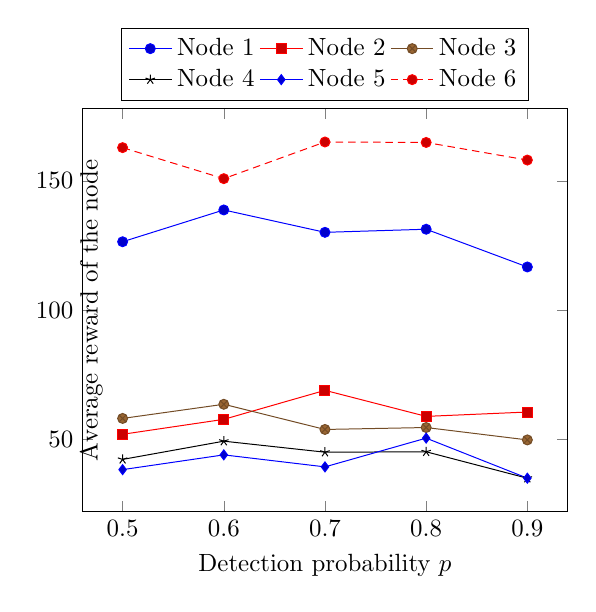
\begin{tikzpicture}[scale=0.9]
\begin{axis}[
  xlabel={Detection probability $p$},
  ylabel={Average reward of the node },
  y label style={at={(0.06,0.5)}},
  xtick={0.5,0.6,0.7,0.8,0.9,1.0},
  legend style={at={(0.5,1.2)},cells={align=right}, anchor=north,legend columns=3},
  grid style=dashed,
]

\addplot+[]
    coordinates {
(0.5,126.469294224)(0.6,138.768688772)(0.7,130.10979383)(0.8,131.308647284)(0.9,116.70873472)
};

\addplot+[]
    coordinates {
(0.5,51.9774584454)(0.6,57.7615872131)(0.7,68.9811633084)(0.8,58.9060250618)(0.9,60.5911805552)
};

\addplot+[]
    coordinates {
(0.5,58.112876005)(0.6,63.5894390224)(0.7,53.8483204974)(0.8,54.5969922461)(0.9,49.8027670671)
};

\addplot+[]
    coordinates {
(0.5,42.2594496478)(0.6,49.3133895991)(0.7,45.0502147208)(0.8,45.20918204)(0.9,34.9808016775)
};

\addplot+[]
    coordinates {
(0.5,38.3055097066)(0.6,44.0188235767)(0.7,39.3680288222)(0.8,50.4912779668)(0.9,34.9978557067)
};

\addplot+[]
    coordinates {
(0.5,162.87848727)(0.6,150.876767477)(0.7,165.06110317)(0.8,164.882126918)(0.9,158.067481047)
};

\legend{Node 1, Node 2, Node 3, Node 4, Node 5, Node 6}
\end{axis}
\end{tikzpicture}

\caption{Scenario c)}
\label{fig:nodeimp_topofullmesh_single}
\end{subfigure}
\begin{subfigure}{.33\textwidth}
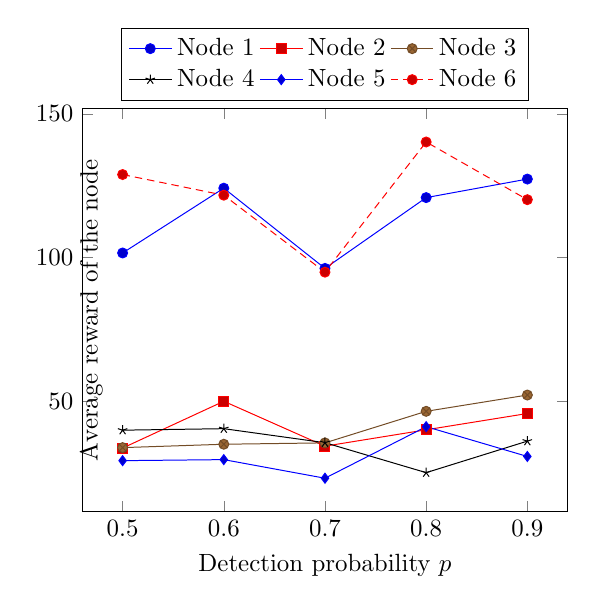
\begin{tikzpicture}[scale=0.9]
\begin{axis}[
  xlabel={Detection probability $p$},
  ylabel={Average reward of the node },
  y label style={at={(0.06,0.5)}},
  xtick={0.5,0.6,0.7,0.8,0.9,1.0},
  legend style={at={(0.5,1.2)},cells={align=right}, anchor=north,legend columns=3},
  grid style=dashed,
]
\addplot+[]
    coordinates {
(0.5,101.616873023)(0.6,124.145242333)(0.7,96.2616914651)(0.8,120.862819291)(0.9,127.305784272)
};

\addplot+[]
    coordinates {
(0.5,33.8037034841)(0.6,50.0693289402)(0.7,34.460597311)(0.8,40.1535742549)(0.9,45.8166364524)
};

\addplot+[]
    coordinates {
(0.5,33.9581528218)(0.6,35.1326808601)(0.7,35.6074089582)(0.8,46.5769811834)(0.9,52.2400544067)
};

\addplot+[]
    coordinates {
(0.5,40.0224063598)(0.6,40.5434953331)(0.7,35.6681036149)(0.8,25.2556265302)(0.9,36.2111392677)
};

\addplot+[]
    coordinates {
(0.5,29.4251886633)(0.6,29.7859232959)(0.7,23.3183642626)(0.8,41.2471235042)(0.9,30.8838558151)
};

\addplot+[]
    coordinates {
(0.5,128.882560148)(0.6,121.704109507)(0.7,94.9489538016)(0.8,140.19719198)(0.9,120.142225907)
};


\legend{Node 1, Node 2, Node 3, Node 4, Node 5, Node 6}
\end{axis}
\end{tikzpicture}

\caption{Scenario d)}
\label{fig:nodeimp_topofullmesh_multiple}
\end{subfigure}
\begin{subfigure}{.5\textwidth}
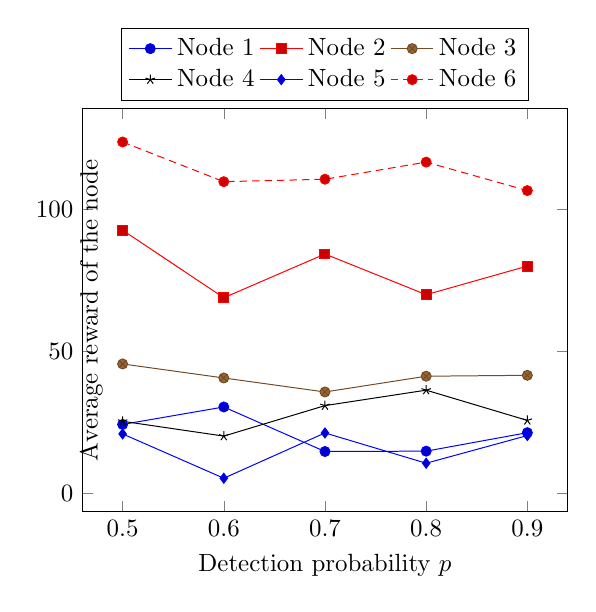
\begin{tikzpicture}[scale=0.9]
\begin{axis}[
  xlabel={Detection probability $p$},
  ylabel={Average reward of the node },
  y label style={at={(0.06,0.5)}},
  xtick={0.5,0.6,0.7,0.8,0.9,1.0},
  legend style={at={(0.5,1.2)},cells={align=right}, anchor=north,legend columns=3},
  grid style=dashed,
]
\addplot+[]
    coordinates {
(0.5,24.2596903238)(0.6,30.4098004181)(0.7,14.7157392372)(0.8,14.8410159329)(0.9,21.3512325325)
};

\addplot+[]
    coordinates {
(0.5,92.6967638225)(0.6,68.892572501)(0.7,84.3050837463)(0.8,69.9668923619)(0.9,80.051680541)
};

\addplot+[]
    coordinates {
(0.5,45.5695982478)(0.6,40.6246377658)(0.7,35.692885081)(0.8,41.2436256503)(0.9,41.5670235599)
};

\addplot+[]
    coordinates {
(0.5,25.3670893308)(0.6,20.1438895136)(0.7,30.888009803)(0.8,36.3312849347)(0.9,25.6728772368)
};

\addplot+[]
    coordinates {
(0.5,20.9174008986)(0.6,5.30161144168)(0.7,21.2602459651)(0.8,10.5837610733)(0.9,20.3331330431)
};

\addplot+[]
    coordinates {
(0.5,123.776293271)(0.6,109.788318837)(0.7,110.653974948)(0.8,116.685625909)(0.9,106.649803871)
};

\legend{Node 1, Node 2, Node 3, Node 4, Node 5, Node 6}
\end{axis}
\end{tikzpicture}

\caption{Scenario e)}
\label{fig:nodeimp_topo2_single}
\end{subfigure}
\begin{subfigure}{.33\textwidth}
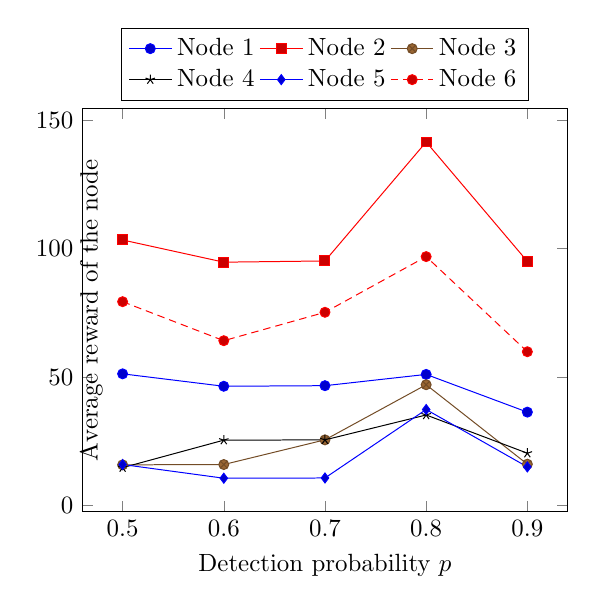
\begin{tikzpicture}[scale=0.9]
\begin{axis}[
  xlabel={Detection probability $p$},
  ylabel={Average reward of the node },
  y label style={at={(0.06,0.5)}},
  xtick={0.5,0.6,0.7,0.8,0.9,1.0},
  legend style={at={(0.5,1.2)},cells={align=right}, anchor=north,legend columns=3},
  grid style=dashed,
]

\addplot+[]
    coordinates {
(0.5,51.2408756424)(0.6,46.3989088055)(0.7,46.629281859)(0.8,51.0165854846)(0.9,36.3262102772)
};

\addplot+[]
    coordinates {
(0.5,103.390154828)(0.6,94.7445634867)(0.7,95.2136135648)(0.8,141.564157095)(0.9,95.0544799628)
};

\addplot+[]
    coordinates {
(0.5,15.7876437463)(0.6,15.9058652472)(0.7,25.5235856726)(0.8,47.0026051031)(0.9,16.0455657836)
};

\addplot+[]
    coordinates {
(0.5,14.6911918445)(0.6,25.4076999562)(0.7,25.5090975344)(0.8,35.2122191081)(0.9,20.3233753667)
};

\addplot+[]
    coordinates {
(0.5,15.9163072098)(0.6,10.573393829)(0.7,10.6704256682)(0.8,37.3424358141)(0.9,14.9838488261)
};

\addplot+[]
    coordinates {
(0.5,79.3520830459)(0.6,64.1507914239)(0.7,75.2190374666)(0.8,96.912552594)(0.9,59.8478399229)
};

\legend{Node 1, Node 2, Node 3, Node 4, Node 5, Node 6}
\end{axis}
\end{tikzpicture}

\caption{Scenario f)}
\label{fig:nodeimp_topo2_multiple}
\end{subfigure}
    \caption{Results for single and multiple attackers}
    \label{fig:mdp-results}
\end{figure}